\documentclass[a4paper,10.5pt]{ltjsarticle}
\usepackage{graphicx}
\usepackage{luatexja-fontspec}
\usepackage{caption}
\usepackage{amsmath,amssymb,bm,braket}
%\usepackage{gnuplot-lua-tikz}
\usepackage[top=10truemm,bottom=15truemm,left=10truemm,right=10truemm]{geometry}
\usepackage{array}
\usepackage{upgreek}
\usepackage{fancyhdr}
\renewcommand{\refname}{}
\usepackage{listings,jvlisting}
\usepackage{tikz}
\usepackage[version=3]{mhchem}
\usetikzlibrary{external}
\tikzexternalize
\lstset{
  basicstyle={\ttfamily},
  identifierstyle={\small},
  commentstyle={\smallitshape},
  keywordstyle={\small\bfseries},
  ndkeywordstyle={\small},
  stringstyle={\small\ttfamily},
  frame={tb},
  breaklines=true,
  columns=[l]{fullflexible},
  numbers=left,
  xrightmargin=0pt,
  xleftmargin=3pt,
  numberstyle={\scriptsize},
  stepnumber=1,
  numbersep=1pt,
  lineskip=-0.5ex
}
\captionsetup[figure]{format=plain, labelformat=simple, labelsep=quad,labelfont=bf}
\captionsetup[table]{format=plain, labelformat=simple, labelsep=quad,labelfont=bf}
\parindent = 0pt
\setmainjfont[BoldFont=HiraMinProN-W6]{HiraMinPro-W3}
%[BoldFont=HGSMinchoE]{MSMincho}[BoldFont=HiraMinProN-W6]{HiraMinPro-W3}
\begin{document}
\centerline{\HUGE \bfseries 物理情報工学CD実験 報告書}
\centerline{ }
\rightline{\vspace{-3mm} \Large 2023年度   }
\begin{table}[h]
  \newcolumntype{I}{!{\vrule width 1.5pt}}
  \newcolumntype{i}{!{\vrule width 0.8pt}}
  \arrayrulewidth=0.8pt
  \renewcommand{\arraystretch}{1.5}
  \newcommand{\bhline}[1]{\noalign{\hrule height #1}}
  \huge
  \centering
  \begin{tabular}{Iwc{6cm}Iwc{2cm}iciwc{5cm}I}
    \bhline{1.5pt}
    実験テーマ&\multicolumn{3}{cI}{A3\ 電子顕微鏡・X線回折技術}\\
    \hline
    担当教員名&\multicolumn{3}{cI}{野村、神原、倉持TA}\\
    \hline
    実験整理番号&80&実験者氏名&平井 優我\\
    \hline
    共同実験者氏名&\multicolumn{3}{cI}{木5班}\\
    \hline
    曜日組&木&実験日&1月11日\\
    \hline
    実験回&9&報告書提出日&1月19日\\
    \bhline{1.5pt}
  \end{tabular}
\end{table}
\clearpage
%1-2-------------------------------------------------------------------------
\hspace{-2pt}{\Large \bfseries 実験課題}\\
{\large \bfseries 1.\ b-1について}\\
 b-1の測定結果を図\ref{fig:b-1}、それらから求まる値を表\ref{tab:b-1}に示す。ただし、Miller指数はAlの計算値の$d$値と比較した結果から求めた。表\ref{tab:b-1}からの$h^2+k^2+l^2$の値から、b-1の結晶は面心立方格子だとわかる。また、表\ref{tab:b-1}の格子定数$a$の推定標準偏差$\delta a$は、$\delta a=2\times10^{-3}\ \mathrm{\AA}$である。よって、推定標準偏差は小さい。このことから、統計誤差は小さいと考えられる。また表\ref{tab:b-1}から、格子定数を求めると、
\begin{align}
  a=4.056(2)\ \mathrm{\AA}
\end{align}
となった。
 これより、実験で得られた値と各金属試料の計算値を比較するとb-1の試料はAlであると推定される。また、Wにおける格子定数の計算値は$4.056\ \mathrm{\AA}$であった。この計算値を真値とすると、系統誤差は、$-3.493\times10^{-4}\ /\ \mathrm{\AA}$となる。\\
\\
{\large \bfseries 2.\ b-2について}\\
 b-2の測定結果を図\ref{fig:b-2}、それらから求まる値を表\ref{tab:b-2}に示す。ただし、Miller指数はWの計算値の$d$値と比較した結果から求めた。表\ref{tab:b-2}からの$h^2+k^2+l^2$の値から、b-1の結晶は体心立方格子だとわかる。また、表\ref{tab:b-2}の格子定数$a$の推定標準偏差$\delta a$は、$\delta a=4.299\times10^{-3}\ \mathrm{\AA}$である。よって、推定標準偏差は小さい。このことから、統計誤差は小さいと考えられる。また表\ref{tab:b-1}から、格子定数を求めると、
\begin{align}
  a=3.174(4)\ \mathrm{\AA}
\end{align}
となった。
 これより、実験で得られた値と各金属試料の計算値を比較するとb-2の試料はWであると推定される。また、Wにおける格子定数の計算値は$3.18\ \mathrm{\AA}$であった。この計算値を真値とすると、系統誤差は、$-6.28\times10^{-3}\ /\ \mathrm{\AA}$となる。\\
\\
{\large \bfseries 3.\ b-3について}\\
 b-3の測定結果を図\ref{fig:b-3}、それらから求まる値を表\ref{tab:b-3}に示す。ただし、Miller指数はCuの計算値の$d$値と比較した結果から求めた。表\ref{tab:b-3}からの$h^2+k^2+l^2$の値から、b-3の結晶は面心立方格子だとわかる。また、表\ref{tab:b-3}の格子定数$a$の推定標準偏差$\delta a$は、$\delta a=1.320\times10^{-2}\ \mathrm{\AA}$である。よって、推定標準偏差は他のb-1、b-2の試料よりも大きい値となった。このことから、統計誤差は大きいと考えられる。また表\ref{tab:b-1}から、格子定数を求めると、
\begin{align}
  a=3.644(13)\ \mathrm{\AA}
\end{align}
となった
 これより、実験で得られた値と各金属試料の計算値を比較するとb-3の試料はCuであると推定される。また、Cuにおける格子定数の計算値は$3.627\ \mathrm{\AA}$であった。この計算値を真値とすると、系統誤差は、$1.757\times10^{-2}\ /\ \mathrm{\AA}$となる。\\
\\
{\large \bfseries 4.\ Sandpaper\_bについて}\\
 Sandpaper\_bの測定結果を図\ref{fig:Sandpaper_b}に示す。実験で得られた$d'$の値と文献\cite{text1}の$d$の値と比較すると、Sandpaper\_bで用いられた物質はSiCのみであるとわかる。\\
\\
{\large \bfseries 5.\ Sandpaper\_wについて}\\
 Sandpaper\_bの測定結果を図\ref{fig:Sandpaper_w}に示す。実験で得られた$d'$の値と文献\cite{text1}の$d$の値と比較すると、Sandpaper\_wで用いられた物質は\ce{Al2O3}のみであるとわかる。\\
\\
{\large \bfseries 6.\ SEMの実験について}\\
 SEMを用いて観察した\ce{YBa2Cu3O7-\gamma}、星砂の画像を図\ref{figure1}、図\ref{figure2}に示す。







\clearpage
\begin{figure}[h]
  \centering
  \includegraphics[scale=0.5,page=2]{b-1.pdf}
  \vspace{-20pt}\caption{b-1の実験値}
  \label{fig:b-1}
\end{figure}
\begin{table}[h]
  \newcolumntype{I}{!{\vrule width 1.5pt}}
  \newcolumntype{i}{!{\vrule width 0.5pt}}
  \arrayrulewidth=0.8pt
  \renewcommand{\arraystretch}{1.5}
  \newcommand{\bhline}[1]{\noalign{\hrule height #1}}
  \centering
  \caption{b-1の$2\theta,\theta,\lambda,d',h^2+k^2+l^2,hkl,a$の値}
  \label{tab:b-1}
  \begin{tabular}{IcicicicicicicI}
    \bhline{1.5pt}
    $2\theta\ /\ ^\circ$&$\theta\ /\ ^\circ$&$\lambda\ /\ \mathrm{\AA}$&$d'\ /\ \mathrm{\AA}$&$h^2+k^2+l^2$&$hkl$&$a\ /\ \mathrm{\AA}$\\
    \bhline{1.0pt}
    38.42&19.21&1.541&2.341&3&111&4.055\\
    44.60&22.30&1.541&2.030&4&200&4.060\\
    65.00&32.50&1.541&1.433&8&220&4.055\\
    65.20&32.60&1.544&1.433&8&220&4.054\\
    78.08&39.04&1.541&1.223&11&311&4.056\\
    78.36&39.18&1.544&1.222&11&311&4.054\\
    \bhline{1.5pt}
  \end{tabular}
\end{table}

\begin{figure}[h]
  \centering
  \includegraphics[scale=0.5,page=2]{b-2.pdf}
  \vspace{-20pt}\caption{b-2の実験値}
  \label{fig:b-2}
\end{figure}
\begin{table}[h]
  \newcolumntype{I}{!{\vrule width 1.5pt}}
  \newcolumntype{i}{!{\vrule width 0.5pt}}
  \arrayrulewidth=0.8pt
  \renewcommand{\arraystretch}{1.5}
  \newcommand{\bhline}[1]{\noalign{\hrule height #1}}
  \centering
  \caption{b-2の$2\theta,\theta,\lambda,d',h^2+k^2+l^2,hkl,a$の値}
  \label{tab:b-2}
  \begin{tabular}{IcicicicicicicI}
    \bhline{1.5pt}
    $2\theta\ /\ ^\circ$&$\theta\ /\ ^\circ$&$\lambda\ /\ \mathrm{\AA}$&$d'\ /\ \mathrm{\AA}$&$h^2+k^2+l^2$&$hkl$&$a\ /\ \mathrm{\AA}$\\
    \bhline{1.0pt}
    40.16&20.08&1.541&2.249&2&110&3.180\\
    58.26&29.13&1.541&1.586&4&200&3.172\\
    73.04&36.52&1.544&1.295&6&211&3.171\\
    73.22&36.61&1.541&1.295&6&211&3.171\\
    \bhline{1.5pt}
  \end{tabular}
\end{table}
\clearpage
\begin{figure}[h]
  \centering
  \includegraphics[scale=0.5,page=2]{b-3.pdf}
  \vspace{-20pt}\caption{b-3の実験値}
  \label{fig:b-3}
\end{figure}
\begin{table}[h]
  \newcolumntype{I}{!{\vrule width 1.5pt}}
  \newcolumntype{i}{!{\vrule width 0.5pt}}
  \arrayrulewidth=0.8pt
  \renewcommand{\arraystretch}{1.5}
  \newcommand{\bhline}[1]{\noalign{\hrule height #1}}
  \centering
  \caption{b-3の$2\theta,\theta,\lambda,d',h^2+k^2+l^2,hkl,a$の値}
  \label{tab:b-3}
  \begin{tabular}{IcicicicicicicI}
    \bhline{1.5pt}
    $2\theta\ /\ ^\circ$&$\theta\ /\ ^\circ$&$\lambda\ /\ \mathrm{\AA}$&$d'\ /\ \mathrm{\AA}$&$h^2+k^2+l^2$&$hkl$&$a\ /\ \mathrm{\AA}$\\
    \bhline{1.0pt}
    42.78&21.39&1.541&2.113&3&111&3.659\\
    49.86&24.93&1.541&1.82&4&200&3.656\\
    50.00&25.00&1.544&1.827&4&200&3.653\\
    73.30&36.65&1.541&1.291&8&220&3.651\\
    73.86&36.93&1.544&1.285&8&220&3.634\\
    89.46&44.73&1.541&1.095&11&311&3.631\\
    89.80&44.90&1.544&1.094&11&311&3.627\\
    \bhline{1.5pt}
  \end{tabular}
\end{table}
\begin{figure}[h]
  \centering
  \includegraphics[scale=0.5,page=2]{Sandpaper_b.pdf}
  \vspace{-20pt}\caption{Sandpaper\_bの実験値}
  \label{fig:Sandpaper_b}
\end{figure}
\begin{figure}[h]
  \centering
  \includegraphics[scale=0.5,page=2]{Sandpaper_w.pdf}
  \vspace{-20pt}\caption{Sandpaper\_wの実験値}
  \label{fig:Sandpaper_w}
\end{figure}
\begin{figure}[h]
  \centering
  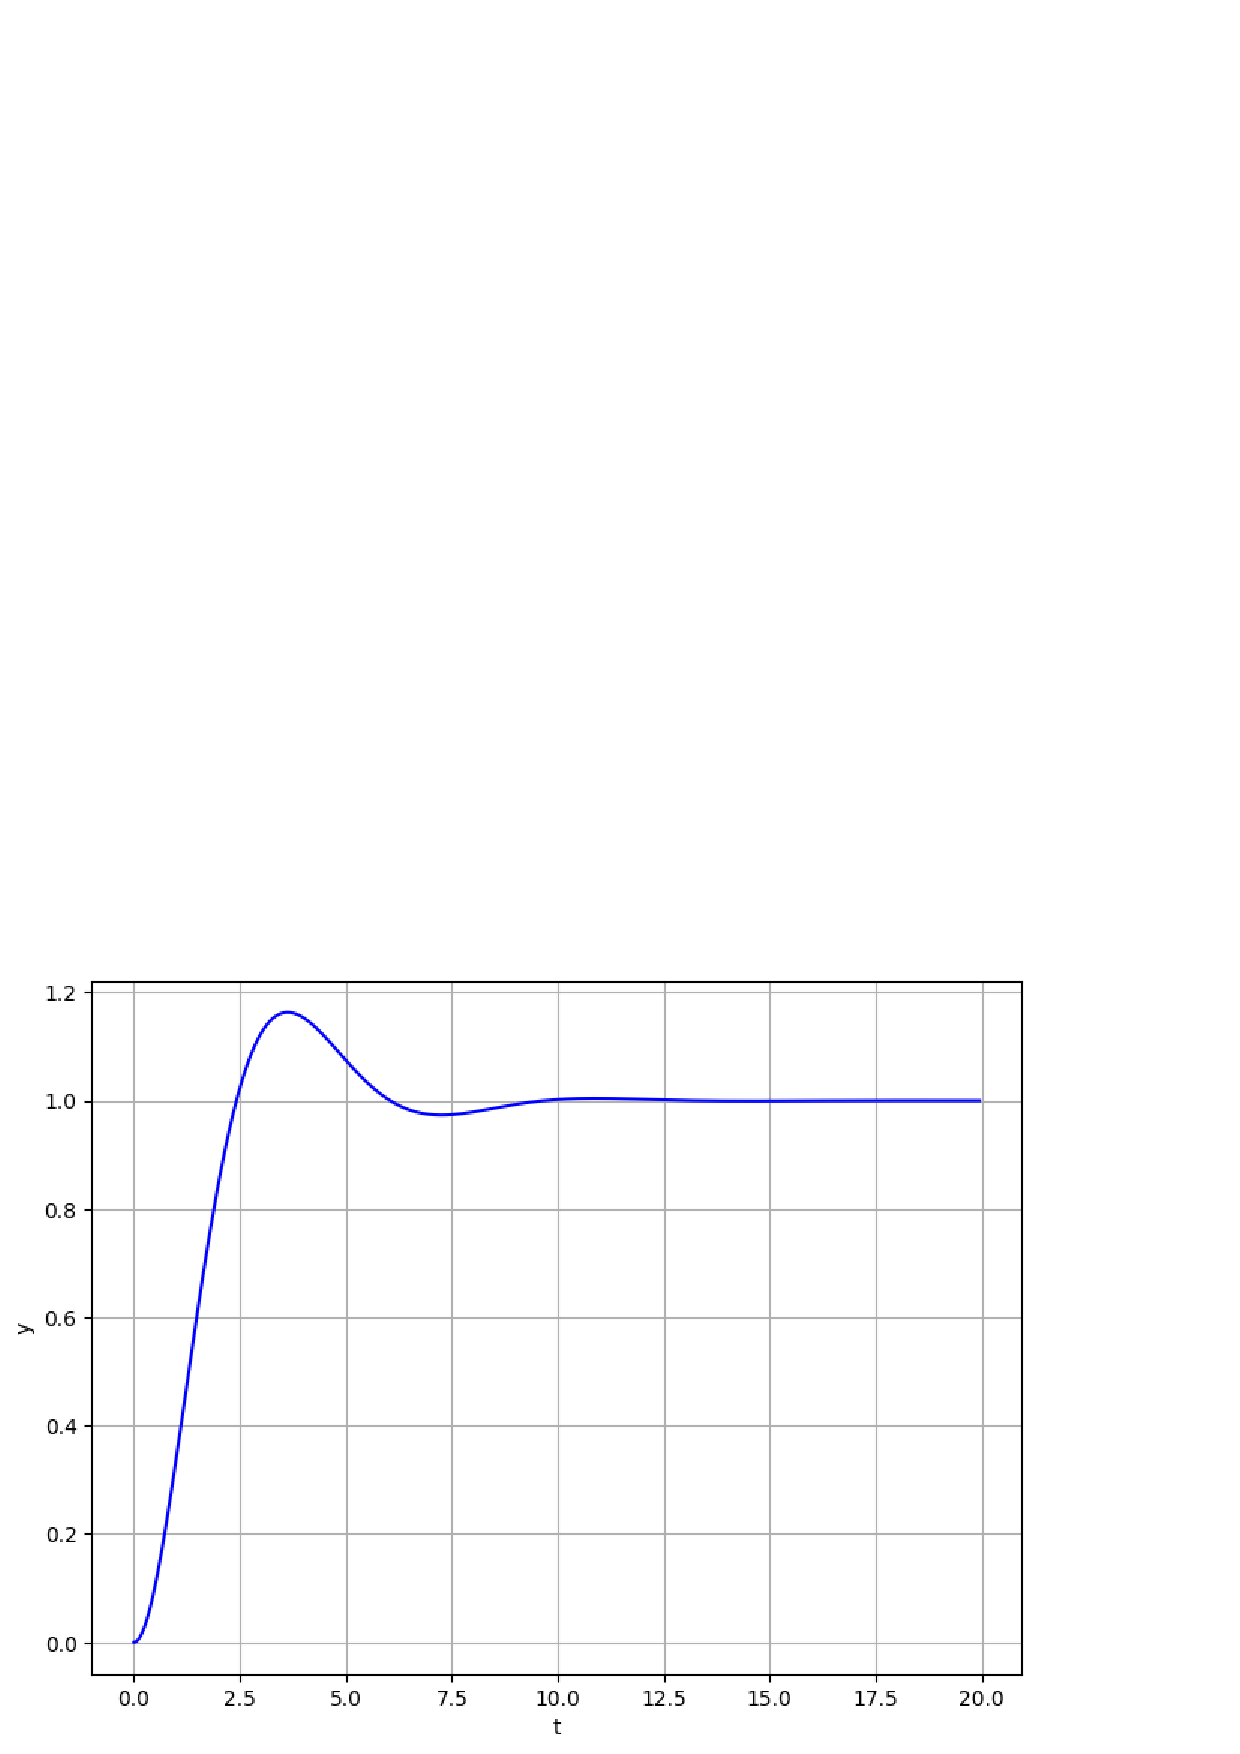
\includegraphics[scale=0.3]{figure2.jpg}
  \caption{\ce{YBa2Cu3O7-\gamma}の表面}
  \label{figure2}
\end{figure}
\begin{figure}[h]
  \centering
  \includegraphics[scale=0.3]{figure1.jpg}
  \caption{星砂の表面}
  \label{figure1}
\end{figure}
\clearpage
{\Large \bfseries 参考文献}
\begin{thebibliography}{1}
\vspace{-1.5cm}
  \bibitem{text} Cu\_Al\_W\_Mo.pdf\ 閲覧日:2024/1/12
  \bibitem{text1} Sandpaper\_data.pdf\ 閲覧日:2024/1/12
\end{thebibliography}
\end{document}
